% ATLAS Mesh Design: furniture that has the shape of the furniture.
% Written by hand; the same text as documents/ATLAS_Mesh_Design.md. Compile with pdflatex, twice (for the page count):
%   pdflatex ATLAS_Mesh_Design.tex && pdflatex ATLAS_Mesh_Design.tex
% The look (fonts, colours, footer) is the one of the other ATLAS handouts.
\documentclass[10pt]{article}
\usepackage[a4paper,top=14mm,bottom=18mm,left=16mm,right=16mm,footskip=9mm]{geometry}
\usepackage[T1]{fontenc}
\usepackage[utf8]{inputenc}
\input{glyphtounicode}\pdfgentounicode=1
\usepackage{helvet}
\renewcommand{\familydefault}{\sfdefault}
\usepackage[varqu,varl]{zi4}
\usepackage[table]{xcolor}
\usepackage{array,booktabs,longtable}
\usepackage{enumitem}
\usepackage{needspace}
\usepackage{listings}
\usepackage{titlesec}
\usepackage{lastpage}
\usepackage[obeyspaces]{url}
\usepackage{tikz}
\usetikzlibrary{arrows.meta}
\usepackage[hidelinks,bookmarksnumbered,pdftitle={ATLAS Mesh Design}]{hyperref}

% ---------- colours (the palette of the other ATLAS handouts) ----------
\definecolor{ink}{HTML}{1F2933}
\definecolor{mute}{HTML}{56616B}
\definecolor{rulec}{HTML}{C9CFD6}
\definecolor{panel}{HTML}{F1F3F5}
\definecolor{laneC}{HTML}{FDEEDE}
\definecolor{laneD}{HTML}{E3EDFC}
\definecolor{accC}{HTML}{9A4A00}
\definecolor{accD}{HTML}{1B55B0}

% ---------- footer ----------
\makeatletter
\def\ps@atlas{%
  \def\@oddhead{}\def\@evenhead{}%
  \def\@oddfoot{\parbox{\textwidth}{\footnotesize\color{mute}ATLAS Mesh Design\hfill 4 October 2026\hspace{6mm}Page \thepage\ of \pageref{LastPage}}}%
  \let\@evenfoot\@oddfoot}
\makeatother
\pagestyle{atlas}

\setlength{\parindent}{0pt}
\setlength{\parskip}{1.8mm}
\color{ink}
\urlstyle{tt}
\newcommand{\cd}{\path}

% ---------- headings ----------
\titleformat{\section}{\fontsize{14.5}{17}\selectfont\bfseries\color{ink}}{\thesection}{0.7em}{}[\vspace{0.6mm}{\color{rulec}\titlerule[0.6pt]}]
\titleformat{\subsection}{\fontsize{11.5}{14}\selectfont\bfseries\color{ink}}{\thesubsection}{0.6em}{}
\titleformat{\subsubsection}{\fontsize{10}{12.5}\selectfont\bfseries\color{accD}}{}{0em}{}
\titlespacing*{\section}{0pt}{6mm}{2.2mm}
\titlespacing*{\subsection}{0pt}{4.2mm}{1.2mm}
\titlespacing*{\subsubsection}{0pt}{3.2mm}{0.6mm}
\setcounter{secnumdepth}{2}

% ---------- lists ----------
\setlist{leftmargin=5mm,itemsep=0.9mm,topsep=0.8mm,parsep=0mm,partopsep=0mm}
\newcommand{\cb}{\raisebox{-0.25ex}{\setlength{\fboxsep}{0pt}\setlength{\fboxrule}{0.7pt}\fcolorbox{mute}{white}{\rule{0pt}{1.75ex}\rule{1.75ex}{0pt}}}\hspace{2mm}}
\newlist{ticks}{itemize}{1}
\setlist[ticks]{label=\cb,leftmargin=7mm,labelsep=0mm,align=left,itemsep=1.4mm,topsep=1.2mm}

% ---------- tables ----------
\newcolumntype{L}[1]{>{\raggedright\arraybackslash}p{#1}}
\newcolumntype{C}[1]{>{\centering\arraybackslash}p{#1}}
\setlength{\tabcolsep}{1.5mm}
\setlength{\LTleft}{0pt}\setlength{\LTright}{0pt}
\setlength{\LTpre}{1.5mm}\setlength{\LTpost}{2.5mm}
\renewcommand{\arraystretch}{1.28}
\newcommand{\hd}[1]{\textbf{#1}}

% ---------- formula blocks ----------
\lstdefinestyle{blk}{basicstyle=\ttfamily\fontsize{8.3}{11.2}\selectfont\color{ink},columns=fullflexible,
  keepspaces=true,upquote=true,showstringspaces=false,backgroundcolor=\color{panel},frame=none,
  aboveskip=4pt,belowskip=4pt,xleftmargin=6pt,framexleftmargin=6pt,breaklines=false}
\lstnewenvironment{blk}{\lstset{style=blk}}{}

% ---------- a panel ----------
\newsavebox{\panelbox}
\newenvironment{panelnote}{\par\vspace{1mm}\begin{lrbox}{\panelbox}\begin{minipage}{\dimexpr\linewidth-6mm\relax}\raggedright}
  {\end{minipage}\end{lrbox}{\setlength{\fboxsep}{3mm}\colorbox{laneD}{\usebox{\panelbox}}}\par\vspace{1mm}}

\begin{document}
\raggedright

{\fontsize{25}{29}\selectfont\bfseries ATLAS Mesh Design\par}
\vspace{1.5mm}
{\fontsize{13}{16}\selectfont\color{mute}Furniture that has the shape of the furniture\par}
\vspace{2.5mm}
{\small\color{mute}4 October 2026. Branch \cd{main}. For the team lead and the three engineers; Appendix A is for
the agents. A design to build now. The decisions in section 2 were taken by the team lead on 4 October 2026. Facts about the
code were read from this tree; anything that could not be checked says so. The same text is in \cd{ATLAS_Mesh_Design.md}.\par}
\vspace{1mm}
{\small\color{mute}Corrected on 4 October 2026 after the first build, so that it says what the code does. Nothing in it has run
on a phone, and the real generator (TripoSG) has never run. When this text was corrected, the Forge's fit, attempts, colour per
face and light copy existed as separate modules (\cd{forge/profile.py}, \cd{forge/colour.py}) and were not yet wired into
clean-up (section 5.3).\par}

% =====================================================================
\section{The problem and the outcome}

\textbf{What is seen today.} Scanned objects stand in the right place and have the right size. Their shape is wrong: a chair
is a generic chair that often faces the wrong way, some objects are plain boxes, and only some look right.

\textbf{Why.} Position and size come from RoomPlan's box, which is good. Shape comes from three places that all fall short:

{\small
\begin{longtable}{@{}L{31mm}L{87mm}L{54mm}@{}}
\toprule
\hd{Seen} & \hd{Cause} & \hd{Where}\\
\midrule
\endhead
Every chair is the same blocky chair & The real generator, TripoSG, has never run. What is shown is the built-in set: box
composites of 22 to about 100 triangles, one per category & \cd{station/forge/forge/generators/triposg.py},
\cd{tools/gen_fallback_set.py}, \cd{ATLAS_Whats_Left.md} item 9\\
It faces the wrong way & An object's yaw is the forward axis of RoomPlan's box, and nothing in our code decides which side of
the box is the front. The built-in chair has its back on local $-$Z whatever the real chair does &
\cd{Scan/Routes/ObjectBoxMerge.cs:54}\\
A generated mesh would face the wrong way too & The Forge turns a mesh by comparing its bounds with the box. That tells
0\textdegree{} from 90\textdegree{} only when the footprint is not square, and never 0\textdegree{} from 180\textdegree. The
phone already sends each photo's camera pose (\cd{camToBox}, \cd{azimuthDeg}); the Forge does not read them &
\cd{forge/cleanup.py:236}, \cd{forge/models.py:35}\\
A plain box & No template for \cd{unknown} and \cd{other}; only the 20 largest objects ever leave their box; a template that
splits past 1,500 triangles is dropped & \cd{tools/gen_fallback_set.py}, \cd{forge/budget.py}, \cd{FallbackMeshBuilder.cs:41}\\
One flat colour & Clean-up picks one palette cell per object from the photo's dominant colour & \cd{forge/cleanup.py:502}\\
No doors or windows & The RoomPlan wall bridge is written and switched off & \cd{Scan/Routes/WallBridge.cs:53}\\
\bottomrule
\end{longtable}}

\begin{panelnote}
\textbf{The outcome.} When this design is built:
\begin{enumerate}[leftmargin=6mm,itemsep=0.7mm,topsep=1mm]
\item Every scanned object has a shape of its own kind the moment the room appears, facing the way the real one faces.
\item Within about a minute per object, that shape is replaced by a mesh generated from the photo of that very object.
\item The mesh sits where the real object is, to the accuracy the scan already has. Accuracy comes first: nothing in this
design moves an object or changes its box.
\item Objects show the colours of their parts, in the palette.
\item A room may hold up to 32 generated meshes and 120,000 furniture triangles, with a lighter copy for the spaces that
cannot afford that.
\item Walls have their real height, doors and windows.
\end{enumerate}
\end{panelnote}

% =====================================================================
\needspace{50mm}
\section{Decisions}

{\small
\begin{longtable}{@{}L{9mm}L{23mm}L{95mm}L{42mm}@{}}
\toprule
\hd{\#} & \hd{Subject} & \hd{Decision} & \hd{Was}\\
\midrule
\endhead
M1 & Purpose & A design to build now, centred on TripoSG producing real furniture shapes & --\\
M2 & Priority & Accuracy first; looks are improved only where accuracy is not put at risk & --\\
M3 & Shape & Two layers: a first shape at once on the phone, then the TripoSG mesh & Box, then mesh or built-in\\
M4 & First shape & Named objects: the category's shape fitted to the scan. Unnamed objects: a shape cut from the scan &
Fixed template, or a box\\
M5 & Facing & Decided from the scan on the phone; the Forge also uses the scan and the photo's camera pose & RoomPlan's box
axis\\
M6 & Disagreement & The generated mesh is always shown, whatever the scan says. The scan chooses its orientation; it never
rejects it & --\\
M7 & Attempts & One generation per object from the best photo. Only when the fit to the scan is poor, the other photos are
tried, and the best fit is shown & One, and one retry on failure\\
M8 & Colour & Per-face palette colours projected from the scan photos. No texture, the one shader & One palette cell per
object\\
M9 & Triangles & Room total 120,000; per object 3,000 to 15,000; up to 32 objects & 60,000; 3,000 to 5,000; 20\\
M10 & Levels & The Forge returns a full and a light copy. Home and Curved Walk show the full one; the other spaces show the
light one until measured & One copy\\
M11 & Room shell & The outline-based shell stays. The RoomPlan wall bridge is turned on for wall heights, doors and windows &
Bridge off\\
M12 & Classification & Stays Apple's (ARKit surface classes, RoomPlan categories). No classifier of our own & Same\\
M13 & Ray casting & Used inside the mesh pipeline (section 6.1). A ray-cast renderer is a future option, sketched in section
6.2 & Not used\\
M14 & Proof & Numbers from a recorded team scan, plus a walk-through on the phone. The record stays on the Station and never
enters git & --\\
M15 & Unchanged & The hosted third-party fallback stays off. The Forge queue stays largest object first & Same\\
\bottomrule
\end{longtable}}

% =====================================================================
\section{How it works after this design}

\vspace{1mm}
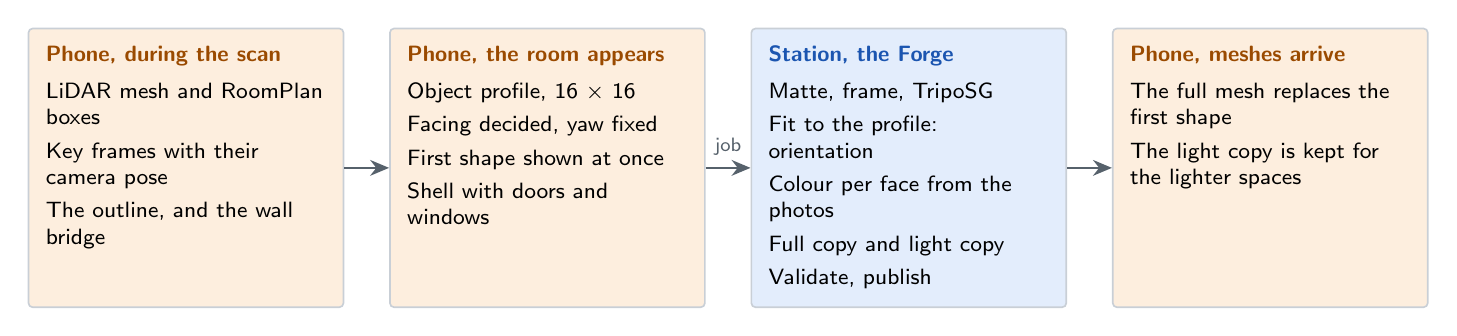
\begin{tikzpicture}[font=\footnotesize,
  box/.style={draw=rulec,line width=0.6pt,rounded corners=1.5pt,inner sep=2.2mm,anchor=north west},
  arr/.style={-{Stealth[length=2.4mm,width=2mm]},line width=0.9pt,color=mute}]
\newcommand{\pbox}[1]{\parbox[t][31mm][t]{35.6mm}{\raggedright #1}}
\node[box,fill=laneC] (a) at (0mm,0) {\pbox{\textbf{\color{accC}Phone, during the scan}\\[1.4mm]
  LiDAR mesh and RoomPlan boxes\\[0.9mm] Key frames with their camera pose\\[0.9mm] The outline, and the wall bridge}};
\node[box,fill=laneC] (b) at (45.9mm,0) {\pbox{\textbf{\color{accC}Phone, the room appears}\\[1.4mm]
  Object profile, 16 $\times$ 16\\[0.9mm] Facing decided, yaw fixed\\[0.9mm] First shape shown at once\\[0.9mm]
  Shell with doors and windows}};
\node[box,fill=laneD] (c) at (91.8mm,0) {\pbox{\textbf{\color{accD}Station, the Forge}\\[1.4mm]
  Matte, frame, TripoSG\\[0.9mm] Fit to the profile: orientation\\[0.9mm] Colour per face from the photos\\[0.9mm]
  Full copy and light copy\\[0.9mm] Validate, publish}};
\node[box,fill=laneC] (d) at (137.7mm,0) {\pbox{\textbf{\color{accC}Phone, meshes arrive}\\[1.4mm]
  The full mesh replaces the first shape\\[0.9mm] The light copy is kept for the lighter spaces}};
\draw[arr] (a.east) -- (b.west);
\draw[arr] (b.east) -- node[above,font=\scriptsize,color=mute,yshift=0.3mm]{job} (c.west);
\draw[arr] (c.east) -- (d.west);
\end{tikzpicture}

Three things are new and carry most of the design:
\begin{itemize}
\item \textbf{The object profile} (section 5.2): a 16 $\times$ 16 grid of heights of the scanned surface inside the object's box.
It is made by casting rays straight down onto the LiDAR mesh. It is tiny, it travels in the RoomModel and in the Forge job,
and it is what decides facing, fits the first shape and orients the generated mesh.
\item \textbf{The fit} (section 5.3): the Forge makes the same profile from the generated mesh and compares the two. The
orientation with the smallest difference wins.
\item \textbf{Two levels} (section 5.4): a full and a light copy of every mesh, so the budget can rise without putting any
space over its limit.
\end{itemize}

% =====================================================================
\needspace{75mm}
\section{Work areas}

For people. Each area is one piece of work with one owner lane. The tasks behind each area are in Appendix A.

{\small
\begin{longtable}{@{}L{35mm}L{64mm}L{11mm}L{35mm}L{21mm}@{}}
\toprule
\hd{Area} & \hd{Delivers} & \hd{Lane} & \hd{Waits for} & \hd{Proved by}\\
\midrule
\endhead
A $\cdot$ TripoSG runs & A real mesh from a real photo, on the Station, in the Forge & D & -- & M2\\
B $\cdot$ Facing and first shapes & The object profile; the facing rule; fitted and scan-cut first shapes; nothing is a plain
box & C, D & -- & M1\\
C $\cdot$ Fit, colour and levels & The Forge orients by the scan, tries again when the fit is poor, colours per face, and
returns two copies & D & A (real meshes), B (the profile), D (the targets) & M2\\
D $\cdot$ The furniture budget & The new triangle rule everywhere it is written; per-space level; the phone measurement &
A, C, D & -- & M3\\
E $\cdot$ Doors and windows & The wall bridge built into the app and switched on & C & -- & M4\\
F $\cdot$ Proof & The recorded scan, the numbers script, the phone checklist & D, lead & A to E & M1 to M4\\
\bottomrule
\end{longtable}}

Areas A, B, D and E do not wait for each other and can be built at the same time. Area C starts on the procedural generator
and the fixtures, and is finished on real meshes once A is through. Area F closes the work.

% =====================================================================
\section{The design}

\subsection{Area A \texorpdfstring{\textperiodcentered}{·} TripoSG runs on the Station}

The adapter (\cd{generators/triposg.py}) was written from the public repository without ever being run. Its calls were checked
against that repository on 4 October 2026 (last upstream commit 18 April 2025; the links are in Appendix C). Nothing was run.
``Read'' means read in the source; ``inferred'' means worked out from it.

{\small
\begin{longtable}{@{}L{24mm}L{70mm}L{23mm}L{52mm}@{}}
\toprule
\hd{Subject} & \hd{What the public repository says} & \hd{Basis} & \hd{What the Forge does}\\
\midrule
\endhead
The calls & The import path, \cd{from_pretrained(dir).to("cuda", float16)}, the call and \cd{.samples[0]} as
\cd{(vertices, faces)} are as the adapter has them & Read & Nothing to change\\
Framing the picture & The picture is cut to the matte's bounding box, put on white and padded to a square by 10\,\% of its
long side on every side. The model's own processor then resizes the short edge to 256 and takes the central
224 $\times$ 224, so a picture that is not square loses its sides & Read & The same framing (below). Today the adapter only puts
the crop on white\\
Matting & Always matted. The model was trained on a foreground that fills 90\,\% of the picture & Read & Matting becomes
required. We use \cd{rembg}; upstream's RMBG-1.4 has a licence of its own\\
Camera angles & Trained on views from the front half of the object, from 15\textdegree{} below to 30\textdegree{} above &
Read (paper) & Photo selection prefers such views (below)\\
The decoder on Windows & The default decoder uses \cd{diso}. One open report: on Windows 10 with Python 3.11 it fails with a
CUDA error and the pipeline then crashes on an empty result & Read; the way round it is inferred and untested & On that
failure the adapter tries again with \cd{use_flash_decoder=False}. \cd{availability()} also checks that \cd{diso} imports\\
Installing & TripoSG's \cd{requirements.txt} pins numpy 1.22.3, which has no build for Python 3.11, the Forge's version.
\cd{transformers} is not pinned: 4.57.0 fails to load the model, 4.56.2 works, the official demo pins 4.49.0 & Read & The
Forge keeps its own pinned list, \cd{requirements-triposg.txt}. The README's install line, which fails as written, is
corrected\\
The weights & 7.95 GB. A folder that was only partly downloaded breaks loading & Read & The adapter looks for
\cd{model_index.json}, not for the folder\\
The result & Vertices inside a cube of $\pm$1.005, with no real-world scale. Shape only: no colour, no texture. The authors'
texturing route needs more memory than this card has and does not run on Windows & Read & Scale to the box as today. Colour
by our own projection (section 5.3)\\
The result's frame & Not documented. The code around it suggests +Y up and the front towards +Z, in the object's own frame
and not the camera's & Inferred & Measured on the first run (below)\\
The result's size & Surfaces are extracted on a 505$^3$ grid; the official demo cuts to 100,000 faces. Raw counts are not
published and are probably several hundred thousand & Read; the count is inferred & Clean-up decimates first, as today, and
its time-out rises from 20~s to 60~s\\
Memory and time & ``At least 8 GB''. One user reports about 9 GB used on a 12 GB card, another about 30 s per mesh. No
official figure, and no report on an RTX 50-series card & Read; user reports & Check M2 measures both on the Station\\
Licences & Code and weights are MIT. \cd{diso} is non-commercial. The decoder taken from FlashVDM is under Tencent's community
licence & Read & Fine for the demo; to be looked at again before any commercial use\\
\bottomrule
\end{longtable}}

\textbf{Set-up.} PyTorch with the cu128 wheels (builds for Python 3.11 exist from 2.7.0), the TripoSG checkout,
\cd{requirements-triposg.txt}, \cd{requirements-gpu.txt}, \cd{FORGE_TRIPOSG_REPO}. \cd{diso} is built from source, so the
Station needs the Microsoft build tools and the CUDA toolkit with \cd{CUDA_HOME} set; without \cd{CUDA_HOME} it builds
without its CUDA part and reports no error. The installed versions and the TripoSG commit go into \cd{docs/versions.md}.

\textbf{What the Forge's first round established beyond the research above} (\cd{station/forge/README.md}, ``First run on
the Station''; nothing here was run on the Station):
\begin{itemize}
\item \textbf{The lock file did not install on Windows.} \cd{requirements.lock} pinned \cd{uvloop} with no platform marker, and
\cd{uvloop} has no Windows build, so \cd{pip install -r requirements.lock} would have failed on the Station. It is now
compiled with \cd{uv pip compile --universal}: \cd{uvloop} is skipped on Windows, \cd{colorama} is added there, and no version
changed.
\item \textbf{\cd{diso} cannot be in a requirements file.} Its build script imports PyTorch and pip builds in an isolated
environment that has none (seen: \cd{ModuleNotFoundError: No module named 'torch'}). It is installed by its own command, after
PyTorch: \cd{pip install setuptools wheel}, then \cd{pip install --no-build-isolation diso==0.1.4} with \cd{CUDA_HOME} set.
\cd{opencv-python} and \cd{pymeshlab}, which only TripoSG's scripts use, are left out of the list.
\item \textbf{The pinned versions.} \cd{torch==2.7.1} and \cd{torchvision==0.22.1} from the cu128 index,
\cd{diffusers==0.33.1}, \cd{transformers==4.49.0}, \cd{huggingface-hub==0.30.2}, \cd{scikit-image==0.25.2},
\cd{scipy==1.15.2}, \cd{peft==0.15.2}, \cd{diso==0.1.4}, \cd{rembg[gpu]==2.0.69}, TripoSG commit
\cd{fc5c40990181e2a756c4e0b1c2f4d6b5202faf8c}. The lists were resolved with \cd{uv pip compile} for Python 3.11 on Windows, and
every pin has a Windows wheel except \cd{antlr4-python3-runtime}, which is pure Python.
\item \textbf{What was tried, and where.} In a throw-away Python 3.11 environment on the build Mac, with PyTorch for the
processor, the TripoSG package imported with \cd{diso} replaced by a stub, and \cd{rembg} cut four of TripoSG's example
pictures, which the Forge framed. No weights were downloaded and nothing was generated. The Windows commands of the run-book are
written from reading, not from running.
\item \textbf{What exists to run it.} The adapter's fallback decoder, the \cd{model_index.json} and \cd{diso} checks, the model
loaded when the service starts, the run-book, \cd{tools/check_station.py} (checks the install) and \cd{tools/first_run.py} (posts
a room and one photo, follows the job, validates the GLB and reads the frame).
\end{itemize}

\textbf{The input picture.} The Forge prepares the crop the way the repository's own script does:
\begin{enumerate}[leftmargin=6mm]
\item Matte the crop. Matting becomes required for the \cd{triposg} generator: \cd{GET /health} reports
\cd{generatorReady: false} when no matting model is installed, instead of sending unmatted room photos to the model.
\item Cut the picture to the matte's bounding box, put it on white, and pad it to a square by 10\,\% of its long side on every
side.
\item Hand that picture to the pipeline. The original crop and its matte are kept in memory for the colour step (section 5.3).
\end{enumerate}

\textbf{The views.} Facing is known when the photos are chosen (section 5.2), so selection can prefer what the model was
trained on: a view's score is halved when the camera stands in the back half of the object, or more than 30\textdegree{}
above its centre. A view from behind is still taken when there is no other.

\textbf{The output frame.} Which way is up, and where the mesh's front is, is measured once on the Station with a test photo
of an object that is clearly not symmetric (a chair seen from the front-left). The answer is set as \cd{triposg_up} and
\cd{triposg_front} in \cd{forge/config.py}; they are settings, read from \cd{FORGE_TRIPOSG_UP} and \cd{FORGE_TRIPOSG_FRONT}
(defaults \cd{Y} and \cd{unknown}) and checked at start-up, and nothing reads them yet because the fit is not wired into
clean-up. \cd{tools/first_run.py} reads the frame from a finished job. \cd{triposg_front} is \cd{canonical} (the front is on the
mesh's own +Z, which after section 5.2 is also the box's front), \cd{view} (the front follows the camera) or \cd{unknown}.
Section 5.3 uses the scan to choose the orientation in any case; this setting only breaks ties.

\textbf{Loading.} The model is loaded when the service starts, not on the first job, so the first object does not pay for it.
\cd{GET /health} reports \cd{generatorReady} only when the load succeeded.

\textbf{Limits.} Generation time-out stays 90 s. The plan's proposal of 60 s per object or less (\cd{P1-D08}) is the figure
check M2 measures.

\subsection{Area B \texorpdfstring{\textperiodcentered}{·} The object profile, facing and first shapes}

\subsubsection{The object profile}

For each object box of a scan that has a real LiDAR mesh (\cd{ScanSnapshot.MeshFromPlanes} is false):
\begin{itemize}
\item \textbf{Grid.} 16 $\times$ 16 cells over the box's footprint in the box's local frame. Cell $(i, j)$ covers local $x$ from
$-w/2 + i\,w/16$ and local $z$ from $-d/2 + j\,d/16$. Index $= 16j + i$, row 0 at the lowest $z$, as the room's distance field.
\item \textbf{Rays.} Four rays per cell (a 2 $\times$ 2 pattern at the quarter points), 1,024 per object. Each starts 0.05 m above
the top of the box and points straight down. It is tested against the scan triangles that overlap the box, floor-class
triangles left out. A hit counts when it lies from 0.02 m above the base to the ray's start.
\item \textbf{Value.} The highest hit of the cell's four rays, as a byte:
\cd{q = clamp(floor(255 * height / h + 0.5), 1, 255)}. \cd{0} means no ray of the cell hit anything.
\item \textbf{Coverage.} Cells that are not 0, divided by 256.
\item \textbf{Where it lives.} \cd{objects[k].profile} in the RoomModel: the 256 bytes as base64 (344 characters). The key is
optional. It is absent for route 1, for a phone without LiDAR, for fixtures, and for an object in which no ray hit anything
(coverage 0); a profile is never stored as 256 zeros. It is not part of the geometry hash.
64 objects add about 23 kB to a file whose limit is 300 kB.
\item \textbf{Where it is made.} \cd{Atlas.Scan}, engine-free, inside \cd{ScanSolver.Solve} on its worker thread, which already
holds the mesh, its classes and the boxes.
\end{itemize}

\subsubsection{Facing}

Facing is decided once, when the RoomModel is built, by the first rule in the object's list that gives an answer. After it,
\textbf{local +Z is the front of every object}: the yaw is turned by whole quarter turns, \cd{size.w} and \cd{size.d} are
swapped on an odd turn, and the profile is turned with them. No reader of the RoomModel needs to change.

{\small
\begin{longtable}{@{}L{20mm}L{84mm}L{68mm}@{}}
\toprule
\hd{Rule} & \hd{Answer} & \hd{Accepted when}\\
\midrule
\endhead
\cd{profile} & The back is the side whose edge strip (the outer 3 of 16 rows) is highest on average; the front is opposite &
That strip has at least a quarter of its cells seen, and its mean height exceeds the next side's by 0.15 of the box height\\
\cd{table} & The front is the side whose outward normal points most towards the centre of the nearest table & A table's box
lies within 1.0 m of the object's box\\
\cd{clearance} & The front is the side with the most free floor in front of it: the room's distance field sampled 0.30 m
outside the middle of each side & The best side exceeds the opposite side by 0.10 m\\
\cd{box} & The box's own axis, as today & Always\\
\bottomrule
\end{longtable}}

{\small
\begin{longtable}{@{}L{105mm}L{70mm}@{}}
\toprule
\hd{Categories} & \hd{Rules, in order}\\
\midrule
\endhead
chair & \cd{profile}, \cd{table}, \cd{clearance}, \cd{box}\\
couch, bed, toilet & \cd{profile}, \cd{clearance}, \cd{box}\\
storage, screen, refrigerator, oven, dishwasher, washerDryer, stove, fireplace, sink, bathtub & \cd{clearance}, \cd{box}\\
table, lamp, plant, stairs, keyboard, mouse, laptop, other, unknown & \cd{box}\\
\bottomrule
\end{longtable}}

\textbf{Ties in \cd{clearance}.} An object's own box limits what any open side can read: the probe is 0.30 m out but the free
region stops one cell (0.05 m) short, so every open side reads at most 0.25 m. A deep appliance against a wall then reads the
same on all three open sides, and ``the most free floor'' is an exact three-way tie, which taken literally goes to the lowest
side: right only when RoomPlan's axis happens to point into the room, and \cd{box} otherwise, which is the case the rule exists
for. So the sides that read within one cell (0.05 m, \cd{ClearanceTie}) of the best count as equally free, and of those the
side that exceeds its opposite side by most is taken. The 0.10 m acceptance is unchanged, and an exact tie that remains (a
square box in a corner) goes to the lowest quarter turn.

\textbf{Two readings} that the table leaves open. In \cd{profile}, ``the next side's'' mean is the highest mean of the other
three strips (a tie gives no answer); the strips share their corner cells, so a scan that saw only the back gives no answer; the
quarter-seen test applies to the highest strip only, so a strip that is highest on a few cells blocks the rule and the next one
answers. In \cd{table}, ``within 1.0 m'' is the distance between the two footprints on the floor, 0 when they overlap; of two
tables equally near the nearer centre wins, and a table that is the object itself gives no answer. In both rules ``exceeds by''
means at least.

The rule that answered is written to \cd{objects[k].facing} (optional key; absent means \cd{box}). Check M1 counts it.

Facing can be switched off by a scan option, \cd{ScanOptions.DecideFacing} (true in \cd{ScanOptions.Default}). With it off the
profile is still computed, because the first shapes and the Forge read it, and only the turning and \cd{facing} are left out. In
this tree \cd{ScanFlow} does not yet hand the option to \cd{ScanSolver.Solve}, so in the app facing is always on; only a direct
call of \cd{ScanSolver.Solve} or \cd{RoomModelBuilder.Build} can switch it off.

\subsubsection{First shapes}

The asset client shows a first shape for every object as soon as the room content is built, not only when the Forge is away.
The mesh state stays \cd{builtIn}; the built-in limit of 1,500 triangles and the 0.25 m edge rule stay.

{\small
\begin{longtable}{@{}L{44mm}L{131mm}@{}}
\toprule
\hd{Object} & \hd{First shape}\\
\midrule
\endhead
chair, couch, bed & The category's template with its measures taken from the profile: seat or mattress height is the median
height of the seen cells in the front half, the back stands on local $-$Z at the height of the box. Defaults are the template's
own when the cells are unseen. The height is kept within 0.25 to 0.70 of the box height for a chair, 0.25 to 0.65 for a couch and
0.30 to 0.75 for a bed (the templates' own are 0.50, 0.45 and 0.55). The fitted shape is the template stretched in height,
piecewise linear, so that the floor, the seat and the top of the box stay where they are and every rectangle of the template
stays a rectangle\\
Other named categories & The fixed template, now facing the right way\\
\cd{unknown}, \cd{other}, and any template that cannot be built & A shape cut from the scan: the profile reduced to
8 $\times$ 8 (the highest of each 2 $\times$ 2), unseen cells filled from their seen neighbours, one column per cell from the floor to
its height, the top and the steps between columns as faces. If that passes 1,500 triangles it is reduced to 4 $\times$ 4.
Tinted by category as the box was\\
No profile, or coverage under 0.30, and no template & The placeholder box. This is the only case left in which a box is seen\\
\bottomrule
\end{longtable}}

The same code builds first shapes on the phone and on the Spectator; the Spectator already reads the whole RoomModel from
the Forge (\cd{SpectatorRooms.cs}), so it has the profile.

\subsection{Area C \texorpdfstring{\textperiodcentered}{·} The Forge fits, colours and levels the mesh}

The job's \cd{meta} gains \cd{profile} (as in the RoomModel) and \cd{triTargetLight}. Clean-up becomes, in order:
\begin{enumerate}[leftmargin=6mm]
\item Weld, decimate to the full target, drop detached fragments (as today, with the new target).
\item \textbf{Orient by the fit.}
\item Scale to the box, at most $\pm$15\,\% of stretch per axis (as today).
\item Regrid so no edge exceeds 0.25 m and the count ends at or below the target (as today).
\item \textbf{Colour per face.}
\item Bake face shade $\times$ ambient occlusion (as today).
\item \textbf{Make the light copy} from the full one: decimate to the light target, then steps 4 to 6.
\item Validate both, publish both.
\end{enumerate}

Clean-up now casts rays and makes two copies, so its time-out rises from 20 s to 60 s.

\subsubsection{The fit}
\begin{itemize}
\item \textbf{Candidates.} The up axes the Forge tries today, times four yaws (0\textdegree, 90\textdegree, 180\textdegree,
270\textdegree), keeping those whose bounds match the box within the stretch limit.
\item \textbf{Score.} For a candidate, the mesh's own profile is made with the same downward rays as section 5.2. The score is
the mean of $|\textrm{generated} - \textrm{scanned}|$ over the cells the scan saw, in fractions of the box height; a cell where
the mesh has no surface counts as height 0. Lower is better; 0 is a perfect match.
\item \textbf{Choice.} The lowest score. When the two best differ by less than 0.02, \cd{triposg_front} breaks the tie:
\cd{canonical} prefers yaw 0\textdegree, \cd{view} prefers the yaw implied by view 0's \cd{camToBox}, \cd{unknown} keeps the
lower score.
\item \textbf{No profile.} \cd{triposg_front} alone decides among the candidates: yaw 0\textdegree{} for \cd{canonical}, the
camera's yaw for \cd{view}. With \cd{unknown}, today's rule.
\item \textbf{Report.} \cd{fit}, \cd{fitYaw}, \cd{fitUp} and \cd{attempts} are added to the clean-up report and to \cd{JobStatus}.
\end{itemize}

\subsubsection{Attempts (decision M7)}

A fit above \textbf{0.20} is poor. The Forge then generates again from view 1, then from view 2, when those exist, and
publishes the attempt with the lowest score. A mesh is always published (decision M6); a poor fit is reported, never hidden.
At most three generations per object.

\subsubsection{Colour per face (decision M8)}
\begin{itemize}
\item For each face and each view: the face is seen when it turns towards the camera (cosine above 0.2), its centre projects
inside the crop, the matte is solid there, and a ray from the camera to the face centre meets no other triangle first. The
crop's own \cd{intrinsics} and \cd{camToBox} give the projection; both are already in the job.
\item The face's colour is the mean of the 5 $\times$ 5 pixels around the projected centre, weighted by the cosine, over the views
that see it.
\item It is mapped to the nearest object cell of the palette (cells 64 to 127), with today's \cd{nearest_entry}.
\item Smoothing: three passes in which a face takes the cell that two of its three neighbours share; then regions under 2\,\%
of the surface merge into their largest neighbour, and the smallest regions merge until at most 6 cells remain.
\item A face no view saw takes the cell of the nearest seen face along the surface. With no seen face at all, the object keeps
one cell from the dominant colour, as today.
\item Vertices are split only where two faces of different cells meet, and every vertex of a face points at the centre of that
face's cell. The shader, the palette and the vertex format do not change. \cd{AssetReady.palette} reports the cell that covers
the most surface.
\end{itemize}

\textbf{Four departures in \cd{forge/colour.py}} (a module with tests; not yet wired into clean-up). Speckle is counted after the
three passes and the 2\,\% merge, not after the limit to 6 cells, because counted after the limit a clean object of eight equal
stripes limited to three cells looks speckled and collapses to one cell. A face no view saw takes the cell of the nearest seen
face by distance along the surface, centre to centre over faces that share a corner or an edge, not by a count of edges crossed,
because the count ran the border between two colours at 45\textdegree{} across an unseen back. After the unseen faces are
filled, the 2\,\% merge and the limit run a second time over the whole mesh, so a small island of seen faces surrounded by unseen
ones cannot survive. And ``no other triangle first'' is an exact ray test from the camera to each face centre, with triangles
binned by their footprint in the picture, not a depth buffer (tolerance 0.01 m; a view that would need more than 12,000,000
ray-triangle tests sees nothing).

\subsubsection{Two levels (decision M10)}
\begin{itemize}
\item The full copy meets the object's full target (section 5.4); the light copy meets the room's light target.
\item \cd{AssetReady} gains \cd{lightSha256}, \cd{lightUrl}, \cd{lightBytes} and \cd{lightTris}. A reader that ignores them
shows the full copy everywhere, as today.
\item \cd{objects[k].assetHashLight} records the light copy beside \cd{assetHash}.
\item The phone downloads the full copy first, since the walker is in Home when meshes arrive, then the light one.
\end{itemize}

\subsection{Area D \texorpdfstring{\textperiodcentered}{·} The furniture budget}

\subsubsection{The rule (decision M9)}

One rule, in whole numbers, so that the phone (\cd{ObjectMeshRules}), the Forge (\cd{budget.py}) and the reference
(\cd{roommath.py}) give the same targets:

\needspace{45mm}
\begin{blk}
N      the objects that receive meshes: the 32 largest by volume, ties to the lower id
a_i    2 * (w*h + h*d + w*d), with w, h, d in whole millimetres: mm(v) = floor(v*1000 + 0.5)
A      the sum of a_i
t_i    clamp( floor(120000 * a_i / A), 3000, 15000 )                the full target of object i
if the sum of t_i is above 120000:
    E = sum of (t_i - 3000)        B = 120000 - 3000*N
    t_i = 3000 + floor( (t_i - 3000) * B / E )
light  clamp( 60000 div N, 1500, 5000 ), whole-number division, the same for every object
\end{blk}

Triangles are shared by surface area, because triangles cover surface. The total never passes 120,000 and no object falls
under 3,000. Objects beyond the 32 largest keep their first shape and have \cd{triTarget} 0.

{\small
\begin{center}
\begin{tabular}{@{}C{38mm}C{30mm}C{26mm}C{30mm}C{26mm}@{}}
\toprule
\hd{Objects of equal size} & \hd{Full target each} & \hd{Full total} & \hd{Light target each} & \hd{Light total}\\
\midrule
5 & 15,000 & 75,000 & 5,000 & 25,000\\
8 & 15,000 & 120,000 & 5,000 & 40,000\\
12 & 10,000 & 120,000 & 5,000 & 60,000\\
20 & 6,000 & 120,000 & 3,000 & 60,000\\
32 & 3,750 & 120,000 & 1,875 & 60,000\\
\bottomrule
\end{tabular}
\end{center}}

\subsubsection{What each copy must satisfy}

{\small
\begin{longtable}{@{}L{27mm}L{55mm}L{55mm}L{29mm}@{}}
\toprule
 & \hd{Full copy} & \hd{Light copy} & \hd{Today}\\
\midrule
\endhead
Triangles & 1,500 to 15,000, and at most the object's target & 1,500 to 5,000, and at most the light target & 1,500 to 5,000\\
File & At most 2 MB & At most 1 MB & 1 MB\\
Longest edge & 0.25 m & 0.25 m & 0.25 m\\
Palette cells & One or more object cells & One or more object cells & One\\
Everything else & \multicolumn{3}{@{}L{145mm}@{}}{As today: one mesh, no material, no texture, 16-bit indices, origin at the base
centre, within 10\,\% of the box}\\
\bottomrule
\end{longtable}}

The worst full copy, every vertex split, is 45,000 vertices of 36 bytes and 90,000 bytes of indices: 1.71 MB.

\subsubsection{Which copy a space shows}

Every space states the level it wants; the room content holds both meshes per object and swaps when a space is entered,
never during a frame.

{\small
\begin{longtable}{@{}L{36mm}L{13mm}L{56mm}L{64mm}@{}}
\toprule
\hd{Space} & \hd{Level} & \hd{Room cost per frame, both eyes} & \hd{New planning row}\\
\midrule
\endhead
S0 Home & Full & 246,000 triangles, 68 draw calls & At most 80 draws and 250k triangles\\
S2 Curved Walk & Full & 246,000 triangles & At most 240 draws and 370k triangles\\
S1, S3, S4, S5, S6 & Light & 126,000 triangles, as today & Triangles as today; 24 more draw calls each, for the 12 more
objects\\
\bottomrule
\end{longtable}}

The must-limits of the plan (300 draw calls and 500,000 triangles per frame) do not change, and every row stays inside them.
Of these rows only Home's is held by code (\cd{RoomBudget}: 80 draw calls and 250,000 triangles per frame, counted from what the
builders make); the others are planning figures until check M3. Three further controls:
\begin{itemize}
\item \textbf{The quality ladder.} The quality table gains one column, furniture level. It is a table in
\cd{Rendering/Quality/QualityFurniture.cs}, not a field of \cd{QualityRow}, which lives in \cd{Atlas.World}. Nominal and High
allow Full; Fair, Serious and Critical force Light in every space, so the first step below nominal drops the furniture to its
light copies before any step lowers the render scale. \cd{QualityApplier.FurnitureCap} and \cd{QualityLadder.FurnitureCap}
publish the column, and \cd{FurnitureLevelPolicy} (\cd{App/Spaces/FurnitureLevels.cs}) puts the resulting level on the room when
a space is entered, when the tier changes, when the parameter changes and when the room is rebuilt.
\item \textbf{A parameter.} \cd{render.furniture} = \cd{auto}, \cd{light} or \cd{full}, so the Console can force a level:
\cd{light} forces Light in every space, \cd{full} forces Full whatever the ladder says.
\item \textbf{The Spectator} always shows the full copy: it downloads no light copy and sets no level.
\end{itemize}

\subsubsection{The measurement (check M3)}

A new fixture, \cd{budget_room_120k}: the room of \cd{budget_room} with 24 stand-ins of exactly 5,000 triangles, 120,000 in
all. On the phone, Home and Curved Walk are run through the existing PerfTour with it. A space that does not hold 60 frames
per second there shows the light copy by default; the full copies are still made for the spaces that hold. Until the
measurement exists, the defaults of the table stand.

\subsection{Area E \texorpdfstring{\textperiodcentered}{·} Doors and windows}

The shell stays as it is: the floor from the confirmed outline, the walls on the outline's edges. That is what makes a
virtual wall coincide with the real one. The wall bridge (\cd{P1-C05}), already written and tested headless, adds what the
shell lacks:
\begin{enumerate}[leftmargin=6mm]
\item \textbf{Build the plugin.} A post-build step, \cd{Editor/AtlasRoomPlanProject.cs} (called from \cd{AtlasPostBuild}), adds
\cd{Plugins/iOS/AtlasRoomPlan.swift} to the sources of the \cd{UnityFramework} target of the generated Xcode project, links the
RoomPlan framework weakly and sets the Swift build settings; applied twice it equals applied once. What was proved: the step was
applied to a copy of an earlier Unity export (made on 3 October 2026, without the Swift file) and the \cd{UnityFramework}
target then built (\cd{BUILD SUCCEEDED}), exporting the four \cd{AtlasRoomPlan} functions with RoomPlan linked weakly. The app
target (\cd{Unity-iPhone}) stopped at its two storyboards, ``iOS 26.1 Platform Not Installed'': the iOS platform component is
not installed on the build Mac. So it is proved that the file and the settings build in a framework target, not that Unity's
export of this tree does, and nothing has run on a phone.
\item \textbf{Switch it on.} \cd{WallBridge.Apply(bool)} sets \cd{WallBridge.Enabled} to the parameter \cd{scan.wallBridge}
(default on; it is the kill switch) and the bridge's own report that it is available. The parameter is not in the on-device
menu's kill-switch list, because the link contract fixes that list as the 21 names of its section 1.5 and a test asserts the
count; it is on the menu's Parameters page.
\item \textbf{Nothing else moves.} A RoomPlan wall still only matches an outline wall; the outline wall keeps its end points.
It takes the height, and its doors, windows and openings. With no capture, an unreadable file or no match, the walls are as
today.
\end{enumerate}

The room's distance field treats every outline edge as a wall, with or without an opening (rule G7), so doors do not change
where the walker may go. \cd{RoomShellBuilder} already cuts openings into walls and kerbs.

\subsection{Area F \texorpdfstring{\textperiodcentered}{·} Proof}

\subsubsection{The record (decision M14)}

One scan of a real room by the team, taken in a session with \cd{FORGE_DEBUG_KEEP=1}. Under the Forge's data folder, which is
already outside git (\cd{station/forge/.gitignore}), it holds: the RoomModel with its profiles, the crops, the generator's raw
output per attempt, the job reports, the published GLBs, and \cd{truth.json}, written once by hand: for each object, which
side is really the front. Because the raw generator output is kept, clean-up can be changed and run again without the GPU.

\cd{tools/meshcheck/check.py} reads the record and prints the numbers below. Only those numbers, and pictures rendered from
the meshes, go into \cd{docs/evidence/mesh/}. No camera frame leaves the Station.

\subsubsection{The checks}

{\small
\begin{longtable}{@{}L{28mm}L{32mm}L{112mm}@{}}
\toprule
\hd{Check} & \hd{Measured on} & \hd{Passes when}\\
\midrule
\endhead
M1 First shapes & The record, and the phone & No object with a profile is a plain box. Facing is right (the correct quarter
turn) for at least 90\,\% of chairs and couches and for every wall-backed object. On the phone the first shapes are there
within 10 s of entering Home\\
M2 Generated meshes & The record & Each of the 32 largest objects has a full and a light copy that pass the validator.
Generation takes 60 s or less per attempt. The median fit is 0.12 or better. Facing is right for at least 90\,\% of objects
that have a front. Every object above 0.20 after its attempts is listed by name\\
M3 Budget & The phone, \cd{budget_room_120k} & Home and Curved Walk hold 60 frames per second with the full copies, or the
space's default is changed to light and the table of section 5.4 is corrected\\
M4 Doors and windows & The phone & In a room with a door and a window, both appear in \cd{walls[].openings}; touching each
side of the door frame is within 5 cm of the drawn edge\\
\bottomrule
\end{longtable}}

\subsubsection{The walk-through on the phone}
\begin{ticks}
\item Every chair faces the way the real chair faces.
\item Nothing in the room is a plain box.
\item Each first shape is replaced by a generated mesh, largest objects first.
\item The generated chair is recognisably that chair, not a chair.
\item Touch points on a table edge and a chair back are as close as they were before this work.
\item An object with two clearly different colours shows both.
\item Entering Aligned Cells and coming back to Home changes the meshes' detail and nothing else.
\item The door and the window are where the real ones are.
\end{ticks}

% =====================================================================
\section{Ray casting}

\subsection{Where rays are used in this design}

{\small
\begin{longtable}{@{}L{40mm}L{52mm}L{44mm}L{33mm}@{}}
\toprule
\hd{Use} & \hd{Rays} & \hd{Against} & \hd{Runs on}\\
\midrule
\endhead
The object profile & 1,024 per object, straight down & The LiDAR mesh inside the box & The phone, at the end of the scan\\
The fit & The same 1,024, per candidate orientation & The generated mesh & The Forge\\
Colour, is this face seen & One per face and view, from the camera & The generated mesh & The Forge\\
Ambient occlusion & 32 directions per vertex (exists today) & The generated mesh & The Forge\\
\bottomrule
\end{longtable}}

None of these runs in a frame. They decide facing, orientation and colour; they do not add detail to a mesh.

\subsection{A ray-cast renderer: a future option}

Not built now. This is what it would be and what would have to be true first.

\textbf{What exists.} Curved space is drawn by moving every vertex with the warp, which places it by the geodesic from the
head: its direction and its length. A straight line of sight from the head is therefore already a geodesic. At every vertex
the picture is exactly what a ray caster would draw. The only error is along an edge between two vertices, which is drawn
straight where the true edge bends, and the 0.25 m edge rule bounds it.

\textbf{What a ray caster would bring.} No edge rule, so no triangles spent only on bending: a table top would no longer need
a grid. Exact depth order on the sphere, where the far side wraps round. It would not add detail to any mesh, and it would
not change where anything stands.

\textbf{What it costs.} Every pixel follows a geodesic into the scene, for two eyes, 60 times a second, on a phone. That is
practical for content given by a formula (the floor and the tiling) and for distance fields. For triangle meshes it needs a
search structure in the shader or hardware ray tracing, and whether Unity offers that on the target phones has not been
checked.

\textbf{A path in three steps, each useful alone.}
\begin{enumerate}[leftmargin=6mm]
\item \textbf{A reference ray caster in the Editor}, on the processor: the exact picture of a test room. It measures the warp's
error in pixels against edge length and distance. If the error is under a pixel beyond some distance, the edge rule can be
relaxed there, which saves triangles with no renderer at all.
\item \textbf{The floor and the tiles per pixel}, in the fragment shader: the tiling is a formula, so a pixel can find its tile
without a mesh.
\item \textbf{Furniture as distance fields}, made by the Forge as a third copy, traced per pixel.
\end{enumerate}

\textbf{Before starting.} Check M3 has shown spare frame time; step 1 has shown an error a person can see; and the support for
step 3 on the phones has been checked.

% =====================================================================
\section{Classification}

Nothing changes (decision M12). For the record, this is who classifies what:

{\small
\begin{longtable}{@{}L{38mm}L{42mm}L{42mm}L{47mm}@{}}
\toprule
\hd{What} & \hd{Classified by} & \hd{Classes} & \hd{Used for}\\
\midrule
\endhead
Triangles of the scan & ARKit's mesh classification & wall, floor, ceiling, table, seat, window, door, none & Free floor,
obstacles, wall directions, and now the object profile (floor triangles are left out)\\
Triangles when the mesh has no classes & Our height and normal test (\cd{ScanSolver.cs:321}) & floor, wall, ceiling, table,
none & The same, on a phone without LiDAR classes\\
Objects & RoomPlan, through AR Foundation's bounding boxes & 23 categories, 16 of which RoomPlan supplies & The tint, the
first shape, the facing rule\\
Obstacle blobs with no RoomPlan box & Nobody: \cd{unknown} & -- & A box today; a scan-cut shape after this design\\
\bottomrule
\end{longtable}}

TripoSG needs no category: it works from the photo. So an \cd{unknown} object gets a generated mesh like any other. Facing is
geometry, not classification.

% =====================================================================
\section{What changes in the frozen contracts}

The contracts were frozen at G0. This design changes them; every edit is listed.

{\small
\begin{longtable}{@{}L{52mm}L{30mm}L{90mm}@{}}
\toprule
\hd{Document or file} & \hd{Section} & \hd{Change}\\
\midrule
\endhead
\cd{documents/ATLAS_Master_Plan.md} & D20, 4.5 & 32 objects, 120,000 triangles, the rule of section 5.4, first shapes, two
levels\\
 & 6.4 asset contract & The table of section 5.4\\
 & 7.4 & Clean-up order of section 5.3; the fit; attempts; colour per face; \cd{AssetReady} light fields\\
 & 8.5 & The rows of section 5.4; the ladder's furniture column\\
\cd{docs/contracts/lane-c-room.md} & 2.1, 2.4 & Optional \cd{profile}, \cd{facing}, \cd{assetHashLight}; \cd{triTarget} 0 or
3,000 to 15,000; local +Z is the front\\
 & 2.7 & R17 follows the new rule; new R21: a profile is exactly 256 bytes\\
 & 2.8 & New rule G14: the profile and facing, after G13\\
 & 9.1, 9.4 & Two meshes per object and a level; first shapes\\
 & 10.1 & Route 4 is on when available\\
 & 11.2 & A view from the back half of the object, or from more than 30\textdegree{} above it, scores half\\
\cd{docs/contracts/roommodel.schema.json} & \cd{objects} & The optional keys; the \cd{triTarget} range\\
\cd{docs/contracts/lane-d-link.md} & 2.5 & \cd{AssetReady} light fields\\
 & 3.6 to 3.9 & \cd{meta.profile}, \cd{meta.triTargetLight}; matting required and the picture framed; the
fallback decoder; the fit; attempts; the report; cleaning time-out 60 s\\
 & 4.1, 4.2 & The table of section 5.4 in both validators\\
 & 4.3, 4.4 & First shapes shown at once; fitted and scan-cut shapes; two downloads per object\\
\cd{docs/contracts/lane-a-platform.md} & 10 & An asset may use several object cells\\
 & Quality table & The furniture column; \cd{render.furniture}\\
\bottomrule
\end{longtable}}

The constants that carry the old numbers: \cd{station/forge/forge/budget.py}, \cd{station/forge/forge/validator.py},
\cd{World/Room/RoomModelValidator.cs:15}, \cd{Telemetry/Assets/GlbValidator.cs:37}, \cd{Rendering/Room/RoomBudget.cs:32},
\cd{tools/rooms/roommath.py}, \cd{tools/rooms/validate_room.py}. The five fixtures are regenerated by
\cd{tools/rooms/make_fixtures.py}; their geometry hashes do not change, because \cd{triTarget}, \cd{profile} and \cd{facing}
are not in the hash.

% =====================================================================
\section{Risks}

{\small
\begin{longtable}{@{}L{66mm}L{109mm}@{}}
\toprule
\hd{Risk} & \hd{What happens then}\\
\midrule
\endhead
TripoSG cannot be made to run on the Station, or is too slow & The number of steps is a setting (the official demo allows 8
to 50). If it still does not hold, another generator goes behind the same interface: Hunyuan3D-2 states 6 GB for shape and
runs on Windows; TRELLIS (16 GB) and SAM 3D Objects (32 GB, Linux) do not fit the card. Until then the first shapes of area B
are what the walker sees, which is already better than today\\
\cd{diso} does not build on the Station, or fails as in the open report & The adapter's fallback decoder. If that fails too,
the row above\\
The generated mesh does not look like the object & It is shown anyway (M6). The fit and the attempts pick the best of three.
The record lists the poor ones so the cause can be found\\
The scan of an object is thin (it was only seen from one side) & Coverage is in the profile. Under 0.30 the profile is not
used for facing or for the first shape; the next rule in the list answers\\
RoomPlan's box axis turns out to be reliable for some category & The record shows it per category; that category's list is
set to \cd{box}\\
The photo and the mesh do not line up, so colours smear & Palette steps and smoothing absorb small errors. If an object ends
up speckled, it falls back to one cell when more than half its faces changed cell during smoothing\\
The full copies are too heavy on the phone & Check M3 switches the space to the light copy, which is today's load\\
The wall bridge cannot share the AR session with the box provider, or does not build & The parameter switches it off and the
walls are as today\\
A second RoomModel reader rejects the new keys & The keys are optional and every reader in the tree ignores unknown keys
except \cd{validate_room.py}, which is changed with the schema\\
\bottomrule
\end{longtable}}

% =====================================================================
\section{Open points}

\begin{enumerate}[leftmargin=6mm]
\item TripoSG's output frame is inferred, not documented (section 5.1), and is measured on area A's first run. The design
works with any of the three settings; the setting only breaks ties.
\item The thresholds are starting values: 0.15 and 0.10 m for facing, 0.20 for a poor fit, 0.30 for coverage, 6 cells per
object. Checks M1 and M2 on the record are where they are tuned.
\item Unity's support for ray tracing on the target phones is unchecked. It matters only for section 6.2, step 3.
\item The two profile implementations differ in one way far below anything measurable. The phone's limits are the float
constants 0.02f and 0.05f widened to double (0.0199999996 and 0.0500000007), and \cd{forge/profile.py} uses 0.02 and 0.05. A hit
within about a nanometre of the 0.02 m limit, or of the ray's start 0.05 m above the top of the box, can count on one side only.
The shared test vectors do not reach it.
\item Three Playground tests fail in the Unity Editor on \cd{main}, for a reason outside this work:
\cd{Blades/Playground/Shell/Cards/HudPanel.cs:117} calls \cd{Destroy} in edit mode. They are not touched by the mesh design and
are listed so that nobody takes them for a failure of it.
\end{enumerate}

% =====================================================================
\appendix
\renewcommand{\thesection}{Appendix \Alph{section}}
\section{Tasks for agents}

One row per task. ``Needs'' lists tasks that must be done first; tasks with none can start at once.

{\footnotesize
\begin{longtable}{@{}L{15mm}L{11mm}L{76mm}L{46mm}L{18mm}@{}}
\toprule
\hd{Task} & \hd{Lane} & \hd{What} & \hd{Done when} & \hd{Needs}\\
\midrule
\endhead
MQ-D01 & D & Install TripoSG from our own pinned list and run one object through the Forge; correct the README's install
line; record versions.\newline \cd{station/forge/requirements-triposg.txt} (new), \cd{station/forge/README.md},
\cd{docs/versions.md} & A GLB from a real photo passes the validator. Built so far: the pinned list, the run-book and
\cd{tools/first_run.py}; the validator has accepted procedural output only, and \cd{docs/versions.md} is not yet written & --\\
MQ-D02 & D & Adapter: the fallback decoder, the checks for \cd{model_index.json} and \cd{diso}, the model loaded at start,
and whatever else the first run shows.\newline \cd{forge/generators/triposg.py},
\cd{forge/service.py} & \cd{GET /health} reports ready; three different photos give three meshes. Built so far: the adapter,
tested with a fake pipeline & MQ-D01\\
MQ-D03 & D & Input picture: matting required, cut to the matte, white, padded square.\newline \cd{forge/imaging.py},
\cd{forge/service.py} & A test photo's prepared picture is square with the object centred & --\\
MQ-D04 & D & Measure and record the output frame.\newline \cd{forge/config.py} & \cd{triposg_up} and \cd{triposg_front} are
set from a non-symmetric test object. Built so far: the two settings (environment variables, defaults \cd{Y} and \cd{unknown})
and the tool that reads the frame & MQ-D02\\
MQ-C01 & C & The object profile in the scan solver.\newline \cd{Scan/Build/ObjectProfile.cs} (new),
\cd{Scan/Routes/ScanSolver.cs} & Synthetic rooms give the expected bytes. Built instead of ``\cd{roommath.py} agrees'': the Forge's \cd{forge/profile.py} and
the phone's \cd{ObjectProfile} pass the same three test vectors (A, B and C of the shared brief, S3); \cd{roommath.py} has no
profile & --\\
MQ-C02 & C & \cd{profile}, \cd{facing}, \cd{assetHashLight} in the RoomModel, the reader, the writer, the schema, rule
R21.\newline \cd{World/Room/RoomModel.cs}, \cd{RoomModelJson.cs}, \cd{RoomModelValidator.cs}, \cd{roommodel.schema.json},
\cd{tools/rooms/} & Round trip on a room with profiles; fixtures still valid & --\\
MQ-C03 & C & The facing rule and the quarter-turn normalisation.\newline \cd{Scan/Build/ObjectFacing.cs} (new),
\cd{RoomModelBuilder.cs} & Synthetic chair, stool, storage, deep-appliance and table cases face as designed, with the tie rule of section 5.2 &
MQ-C01, MQ-C02\\
MQ-C05 & C & Photo selection prefers views from the front half and from no more than 30\textdegree{} above.\newline
\cd{Scan/Photo/PhotoScore.cs} & Of a front and a back view of equal quality, the front one is view 0 & MQ-C03\\
MQ-D05 & D & Fitted templates for chair, couch and bed; the scan-cut shape.\newline
\cd{Telemetry/Assets/FallbackMeshBuilder.cs}, \cd{FittedShapes.cs} (new), \cd{tools/gen_fallback_set.py} & Every category and
\cd{unknown} build under 1,500 triangles, no edge over 0.25 m & MQ-C02\\
MQ-D06 & D & First shapes shown at once, on the phone and the Spectator.\newline \cd{Telemetry/Assets/AssetClientCore.cs},
\cd{Spectator/SpectatorFurniture.cs} & With the Forge reachable, no object that has a template or a usable profile is a box after the room is built & MQ-D05\\
MQ-A01 & A, C, D & The triangle rule in all three places, and the validators.\newline \cd{RoomModelValidator.cs},
\cd{forge/budget.py}, \cd{tools/rooms/roommath.py}, \cd{GlbValidator.cs}, \cd{forge/validator.py} & The table of section 5.4
from all three; the fixtures regenerate & --\\
MQ-D07 & D & The fit: the mesh's profile, candidates, choice, report; cleaning time-out 60 s.\newline \cd{forge/cleanup.py},
\cd{forge/profile.py} (new), \cd{forge/models.py}, \cd{forge/config.py} & A test mesh turned by each quarter turn is turned back. Built so far: \cd{forge/profile.py} with its tests (the mesh's profile,
the fit score, the turning); the fit is not yet in clean-up & MQ-C02\\
MQ-D08 & D & Attempts on a poor fit.\newline \cd{forge/service.py} & A forced poor fit runs views 1 and 2 and publishes the
best & MQ-D07\\
MQ-D09 & D & Colour per face.\newline \cd{forge/colour.py} (new), \cd{forge/cleanup.py}, \cd{forge/palette.py} & A two-colour
test object gives two cells in the right places. Built so far: \cd{forge/colour.py} with its tests, which include a two-colour
object; it is not yet in clean-up & MQ-D07\\
MQ-D10 & D & The light copy; \cd{AssetReady} light fields; two downloads.\newline \cd{forge/cleanup.py},
\cd{forge/service.py}, \cd{Link/Messages/JsonMessages.cs}, \cd{AssetClientCore.cs} & Both copies validate; an old reader
still shows the full one. Built so far: the phone's side (the message fields, the Hub pass-through, the validator levels, the
light download) and the Forge's validator and \cd{JobStatus} fields; the Forge does not yet make a light copy & MQ-A01\\
MQ-A02 & A, C & Two meshes per object and a level in the room content; each space's level; the ladder column;
\cd{render.furniture}.\newline \cd{World/Room/IRoomContent.cs}, \cd{Rendering/Room/RoomContent.cs}, \cd{Rendering/Quality/},
the space modules & Entering a light space swaps meshes; the ladder's first step forces light & MQ-D10\\
MQ-A03 & A & \cd{budget_room_120k} and the budget tests.\newline \cd{tools/rooms/make_fixtures.py},
\cd{Rendering/Room/RoomBudget.cs}, tests & \cd{RoomBudget.Estimate} gives about 246,000 triangles per frame for Home (tested within 5,000 of it, the shell being a few
thousand) and 52 draw calls for the 24 stand-ins & MQ-A01\\
MQ-C04 & C & Build the Swift plugin into the Xcode project; switch the bridge on.\newline
\cd{Plugins/iOS/AtlasRoomPlan.swift}, an Editor post-build step, \cd{Scan/Routes/WallBridge.cs}, \cd{App/Params/AppParams.cs}
(\cd{Atlas.Scan} cannot reach the registry, so the parameter is declared there) & The app builds; \cd{scan.wallBridge} turns it
off. Built so far: the post-build step, tested headless, and the \cd{UnityFramework} target built from a copy of an earlier
export; the app target stopped at storyboards on this Mac (section 5.5); the parameter is tested headless & --\\
MQ-F01 & D & The record and \cd{tools/meshcheck/check.py}; raw generator output kept under debug-keep.\newline
\cd{forge/service.py}, \cd{tools/meshcheck/} (new) & The script prints the numbers of M1 and M2 from a record & MQ-D07\\
MQ-F02 & Lead & Take the record; write \cd{truth.json}; run M1 to M4; fill \cd{docs/evidence/mesh/} & The four checks have a
result each & All\\
\bottomrule
\end{longtable}}

\section{Formulas}

\textbf{Yaw and the quarter turns.} Yaw $\psi$ turns local +Z towards local +X (lane C contract, section 1). If the front is
found on local +X, the new yaw is $\psi + \pi/2$; on local $-$Z, $\psi + \pi$; on local $-$X, $\psi - \pi/2$; each wrapped to
$(-\pi, \pi]$. On +X and $-$X, \cd{size.w} and \cd{size.d} swap. The profile is turned by the same number of quarter turns so
that its row 15 is the front.

\textbf{Side strips of the profile.} Back strip of the candidate front +Z: rows $j = 0$ to 2. Of +X: columns $i = 0$ to 2. Of
$-$Z: rows 13 to 15. Of $-$X: columns 13 to 15. A strip's mean is over its seen cells, as height $\div$ box height.

\textbf{The fit score.} With $S$ the cells the scan saw, $p$ the scanned profile and $g$ the generated mesh's, both as fractions
of the box height, and $g = 0$ where the mesh has no surface:
\[ \textrm{score} = \frac{1}{|S|} \sum_{c \in S} |g_c - p_c| . \]

\textbf{The view's yaw.} With \cd{camToBox} the camera-to-box transform of view 0, the camera stands at $c$, its translation.
The azimuth of the view is $\mathrm{atan2}(c_x, c_z)$ in the box's frame; the nearest quarter turn to it is the candidate the
tie-break prefers when \cd{triposg_front} is \cd{view}. Its elevation is the angle of $c - (0, h/2, 0)$ above the horizontal.

\section{Where things are}

{\small
\begin{longtable}{@{}L{58mm}L{117mm}@{}}
\toprule
\hd{Subject} & \hd{File}\\
\midrule
\endhead
The scan routes, the solver & \cd{ATLAS/Assets/Atlas/Scan/Routes/ScanSolver.cs}, \cd{ScanSession.cs}\\
RoomPlan boxes to object boxes & \cd{ATLAS/Assets/Atlas/Scan/Routes/ObjectBoxMerge.cs}\\
The RoomModel & \cd{ATLAS/Assets/Atlas/World/Room/}, \cd{docs/contracts/lane-c-room.md}\\
Photo capture and what is sent & \cd{ATLAS/Assets/Atlas/Scan/Photo/}, \cd{World/Room/IObjectPhotoSink.cs},
\cd{Telemetry/Assets/ForgeTransport.cs}\\
The Forge & \cd{station/forge/} (\cd{service.py}, \cd{cleanup.py}, \cd{budget.py}, \cd{validator.py}, \cd{generators/})\\
The asset client and the built-in set & \cd{ATLAS/Assets/Atlas/Telemetry/Assets/}\\
The room as drawn & \cd{ATLAS/Assets/Atlas/Rendering/Room/}\\
The warp and the room in curved space & \cd{Rendering/Shaders/Resources/AtlasWarp.hlsl},
\cd{Rendering/Tiles/CurvedRoomView.cs}\\
The wall bridge & \cd{ATLAS/Assets/Atlas/Scan/Routes/WallBridge.cs}, \cd{ATLAS/Assets/Plugins/iOS/AtlasRoomPlan.swift}\\
\bottomrule
\end{longtable}}

\textbf{Outside the tree} (read on 4 October 2026; nothing was run):

{\small
\begin{longtable}{@{}L{58mm}L{117mm}@{}}
\toprule
\hd{Subject} & \hd{Source}\\
\midrule
\endhead
TripoSG: the inference script, the framing, the pipeline, the requirements & \url{https://github.com/VAST-AI-Research/TripoSG}
(\cd{scripts/inference_triposg.py}, \cd{scripts/image_process.py}, \cd{triposg/pipelines/pipeline_triposg.py},
\cd{requirements.txt})\\
TripoSG: the weights, their size and licence & \url{https://huggingface.co/VAST-AI/TripoSG}\\
TripoSG: training views, the 90\,\% foreground & \url{https://arxiv.org/abs/2502.06608} (sections 5.1 and 5.2.1)\\
The decoder failing on Windows & \url{https://github.com/VAST-AI-Research/TripoSG/issues/63}\\
The \cd{transformers} version that fails & \url{https://github.com/VAST-AI-Research/TripoSG/issues/61}\\
\cd{diso}: built from source, its licence & \url{https://github.com/SarahWeiii/diso}\\
Other generators, for the risk table & \url{https://github.com/Tencent-Hunyuan/Hunyuan3D-2},
\url{https://github.com/microsoft/TRELLIS}, \url{https://github.com/facebookresearch/sam-3d-objects}\\
\bottomrule
\end{longtable}}

\end{document}
